\begin{frame}
    \titlepage
\end{frame}

\begin{frame}{Outline}
    \tableofcontents
\end{frame}

\section{Charge density prediction and equivariant neural networks}

\begin{frame}{What is Charge Density?}
    \begin{itemize}
        \item Charge density $\rho(\mathbf{r})$ represents the probability distribution
        of electrons in a system
        \begin{equation*}
            \rho(\mathbf{r}) = N\int |\Psi(\mathbf{r}, \mathbf{r}_2, \cdots, \mathbf{r}_N)|^2
            d\mathbf{r}_2 \cdots d\mathbf{r}_N,
            \quad \rho(\mathbf{r}) = \sum_{i=1}^N |\phi_i(\mathbf{r})|^2,
        \end{equation*}
        for Hartree–Fock and density functional theory (DFT) where orbitals are defined.
        \item Key properties:
        \begin{itemize}
            \item Non-negative: $\rho(\mathbf{r}) \geq 0$.
            \item Normalized: $\int \rho(\mathbf{r}) d\mathbf{r} = N$ (number of electrons).
        \end{itemize}
    \end{itemize}
    \begin{figure}
        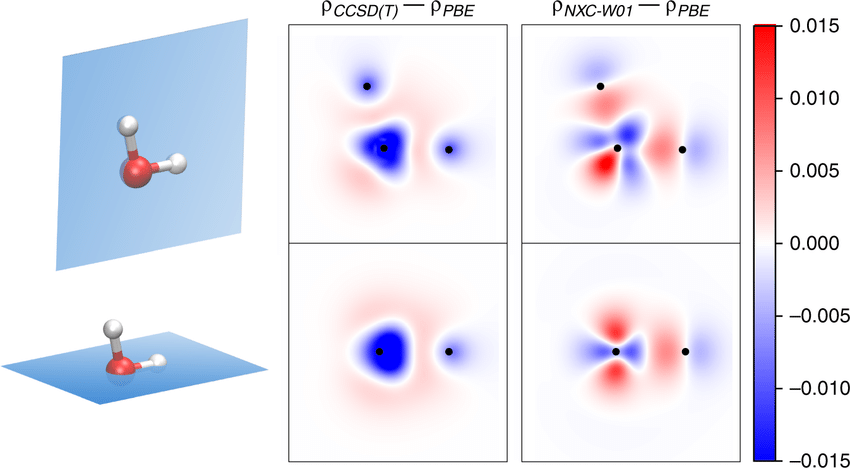
\includegraphics[width=0.5\textwidth]{figures/water_electron_density.png}
    \end{figure}
\end{frame}

\begin{frame}{Why is Charge Density Important?}
    \begin{itemize}
        \item Fundamental quantity of the DFT, required for
        most downstream calculations:
            \begin{itemize}
                \item Band structure, phonon properties, etc.
                \item High-throughput screening
                \item Property optimization \& Structure prediction
            \end{itemize}
        \item Contains more information than the energy and force prediction. For a system
        with $N$ atoms.
        \begin{itemize}
            \item Total energy + Forces: dimension = $3N + 1$.
            \item Charge density: dimension = $n^3$ ($n$ is the plane-wave grid size) or
            the number of basis functions.
            \item An analog: Text2Text v.s. Text2Image.
        \end{itemize}
    \end{itemize}
\end{frame}

\begin{frame}{Challenges in Charge Density Prediction}
    Physical constraints:
    \begin{itemize}
        \item E(3) = O(3) $\oplus \ \mathbb{R}^3$ equivariance: given two systems $\{(\mathbf{r}_a, Z_a)\}$ and
        $\{(\mathbf{r}_a', Z_a')\}$
        related by $\mathbf{r}_a^{\prime} = \operatorname{R}\mathbf{r}_a + \mathbf{t}, Z_a^{\prime} = Z_a$, the
        charge density should satisfy:
        \begin{equation*}
            \rho(\mathbf{r}) = \rho'(\operatorname{R}\mathbf{r} + \mathbf{t}), \quad
            \operatorname{R} \in \operatorname{O}(3), \mathbf{t} \in \mathbb{R}^3.
        \end{equation*}
        {\color{red}\textbf{Much more difficult than the energy and force prediction,
        especially for the rotational equivariance. Equivariance on the level of operator.}}
        \item If $E = E(\{(\mathbf{r}_a, Z_a)\})$ is G-invariant, then the gradient
        of it $F = \nabla_{\mathbf{r}_a}E(\{(\mathbf{r}_a, Z_a)\})$ is G-equivariant.
    \end{itemize}
\end{frame}

\begin{frame}{Two network parametrization for equivariance}
    \begin{itemize}
        \item (Basis-based) For molecular systems with basis functions, we require:
        \begin{align*}
            \rho(\mathbf{r}) &= \sum_{a} \sum_{l=0}^{\infty} \sum_{m=-l}^{l} c_{alm}
            R_{al}(|\mathbf{r} - \mathbf{r}_a|)Y_{lm}(\widehat{\mathbf{r} - \mathbf{r}_a}), \quad r = |\mathbf{r}|,
            \quad \widehat{\mathbf{r}} = \frac{\mathbf{r}}{r}.
        \end{align*}
        The equivariance of the density can be expressed as the equivariance of the
        vector of coefficients $c_{alm}$.
        \begin{equation*}
            \{(\mathbf{r}_a, Z_a)\} \rightarrow \{c_{alm}\}
        \end{equation*}
        \item (Probe-based) For general systems, motivated by implicit neural representation, we
        require the following map to be invariant:
        \begin{equation*}
            \{(\mathbf{r}_a, Z_a), \mathbf{r}_1^{\prime}, ..., \mathbf{r}_n^{\prime}\} \rightarrow
            \{\rho(\mathbf{r}_1^{\prime}), \rho(\mathbf{r}_2^{\prime}), ..., \rho(\mathbf{r}_n^{\prime})\}.
        \end{equation*}
        \item (Mesh-based) Mesh representation of density can model the translational equivariance
         but not the rotational equivariance.
    \end{itemize}
\end{frame}


\begin{frame}{Representation of SO(3): spherical harmonics}
    \begin{itemize}
        \item Spherical harmonics $Y_{lm}(\hat{\mathbf{r}})$ are eigenfunctions of
        angular momentum operators.
        \item $\{Y_{lm}\}_{m=-l}^l$ forms
        an irreducible representation of SO(3) of dimension $2l+1$.
        \begin{equation*}
            Y_{lm}(\operatorname{R}\hat{\mathbf{r}}) = 
            \sum_{m'=-l}^{l} D_{m'm}^l(\operatorname{R}) Y_{lm'}(\hat{\mathbf{r}})
            \Longrightarrow (\operatorname{R}c)_{lm} = \sum_{m'=-l}^{l}
            D_{m'm}^l(\operatorname{R}) c_{lm'}.
        \end{equation*}
    \end{itemize}
    \begin{figure}
        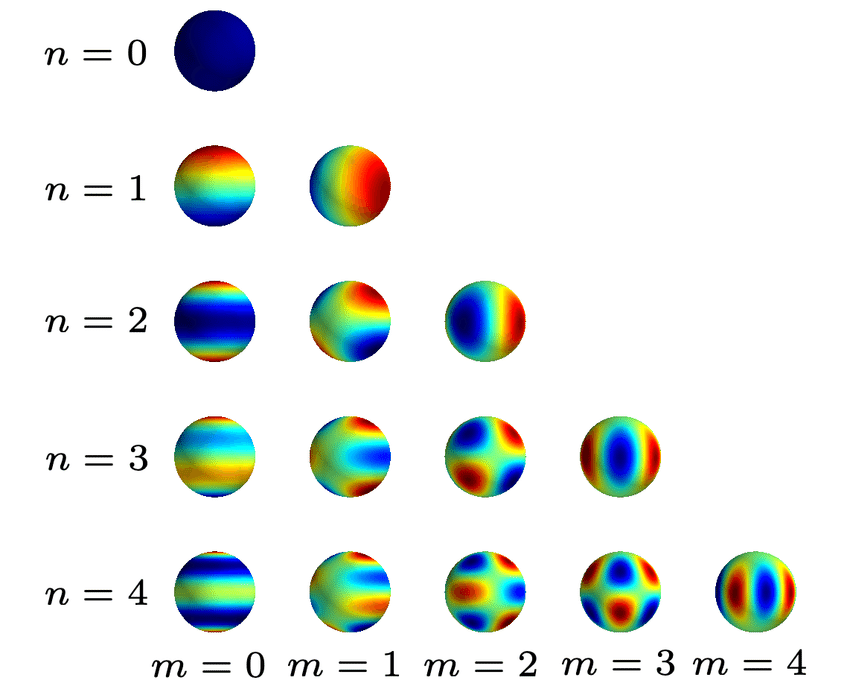
\includegraphics[width=0.45\textwidth]{figures/sh.png}
    \end{figure}
\end{frame}


\begin{frame}{Add equivariance into graph neural networks (GNN)}
    \begin{itemize}
        \item A GNN is defined on a graph $\mathcal{G} = (\mathcal{V}, \mathcal{E})$
        is permutation equivariant.
        \item A series of functions
        $f: \mathbb{R}^{|\mathcal{V}| \times F_i} \rightarrow \mathbb{R}^{|\mathcal{V}| \times F_{i+1}}$,
        locally aggregates all the features belonging to the neighborhood. For example,
        a GCN layer:
        \begin{equation*}
            f(X) = \sigma(D^{-1/2}\widetilde{A}D^{-1/2}XW), \quad 
            A, D \in \mathbb{R}^{|\mathcal{V}| \times |\mathcal{V}|}, X \in \mathbb{R}^{|\mathcal{V}| \times F_i},
            W \in \mathbb{R}^{F_i \times F_{i+1}}, \widetilde{A} = A + I,
        \end{equation*}
        where $W$ is the learnable weight matrix.
    \end{itemize}
    To enforce the equivariance $\text{NN}(gX) = g\text{NN}(X), g \in G$:
    \begin{itemize}
        \item The set of features $X$ should have a SO(3)-action: construct $X$ via 
        spherical harmonics.
        \item The function $f$ should be equivariant for each layer: special attention
        on the architecture design.
    \end{itemize}
\end{frame}


\begin{frame}{Build an equivariant GNN: irreps as features}
    \begin{itemize}
        \item For each graph node, the feature vector is the direct sum of all the irreps of dimension
        less than or equal to $L$.
        \item Invariant scalar corresponds to $l=0$; vector corresponds to $l=1$; below
        is the transformation matrix of a rotation on reps 10x0o + 5x01o + 5x02o.
    \end{itemize}
    \begin{figure}
        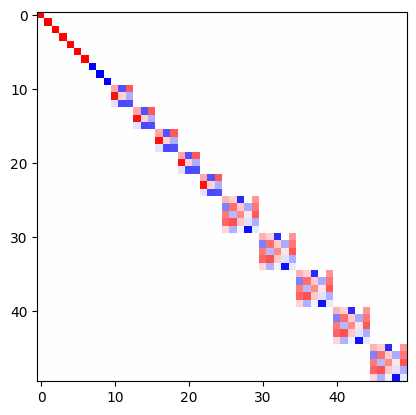
\includegraphics[width=0.4\textwidth]{figures/irreps.jpg}
    \end{figure}
\end{frame}
 

\begin{frame}{Fully Connected Tensor Product Operation}
    \begin{itemize}
        \item Mathematical definition: reps = reps1 $\otimes$ reps2.
        \begin{align*}
            (U^{(l_1)} \otimes V^{(l_2)})^{(l)}_{cm} &=
            \sum_{m_1=-l_1}^{l_1} \sum_{m_2=-l_2}^{l_2}
            C^{(l,m)}_{(l_1,m_1)(l_2,m_2)} U^{(l_1)}_{cm_1}
            V^{(l_2)}_{cm_2},
        \end{align*}
        where $|l_1 - l_2| \leq l \leq |l_1 + l_2|$,
        $C^{(l,m)}_{(l_1,m_1)(l_2,m_2)}$ are Clebsch-Gordan coefficients
        \item {\color{red}\textbf{Equivariant convolution combines features of different angular momenta}}:
        \begin{align*}
            \text{Conv}(\mathbf{r}_a, V_{alm}^c) &=
            \sum_{m_1, m_2}
            C^{(l,m)}_{(l_1,m_1)(l_2,m_2)} \sum_{b \in \partial a}
            V_{bl_1m_1}^c R(r_{ab})Y_{l_2m_2}(\hat{\mathbf{r}}_{ab}),   \\
            R(r_{ab}) &= W_n\sigma(\cdots \sigma(W_2\sigma(W_1 B(r_{ij})))), \quad
            B(r_{ab}) = \frac{2}{r_c}\frac{\sin(\frac{n\pi}{r_c}r_{ij})}{r_{ij}}
            f(r_{ij}, r_c).
        \end{align*}
        \item Equivariance follows from the definition of the tensor product of the
        reps and the second reps depends both on the parameters and $\mathbf{r}$.
    \end{itemize}
\end{frame}


\begin{frame}{Equivariant graph convolution}
    \begin{figure}
        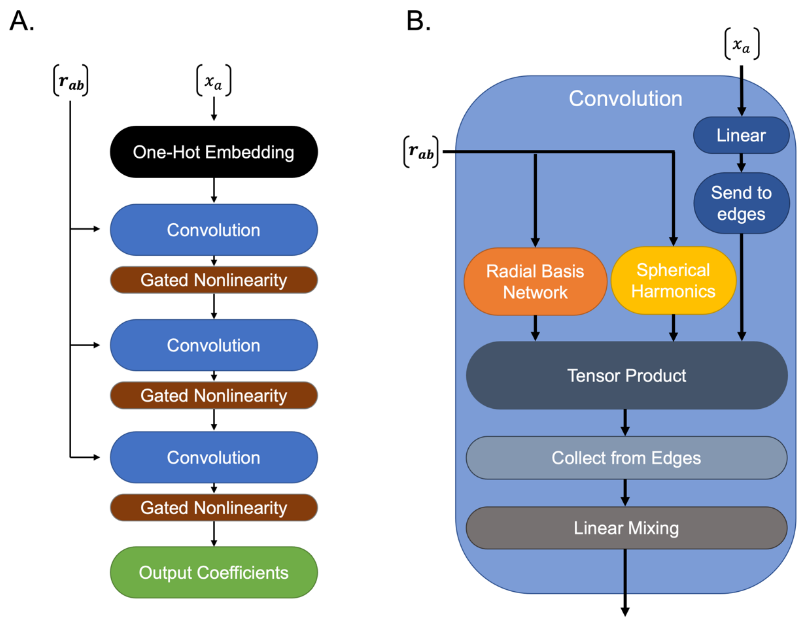
\includegraphics[width=0.6\textwidth]{figures/e3nn_1.jpg}
    \end{figure}
\end{frame}


\begin{frame}{Other equivariant operations}
    \begin{itemize}
        \item Gated nonlinearity:
        \begin{equation*}
            \sigma_{\text{Gated}}(X) = \sigma(X_{l=0}) \oplus (\sigma(X_{l=0})
            \cdot X_{l \neq 0}).
        \end{equation*}
        \item Self-interaction (similar to $1\times 1$ convolution)
        \begin{equation*}
            X_{c_1l}^{\text{out}} = \sum_{c_2} W_{c_1c_2}X_{jl}^{\text{in}}, \quad c_1 \in [F_{\text{out}}],
            c_2 \in [F_{\text{in}}], l \in [(L + 1)^2].
        \end{equation*}
        \item Point-wise spherical non-linearity.
        \item Selfmix layers (similar to self-attention), tensor product with itself.
        \item Pairmix layers.
    \end{itemize}
\end{frame}


\begin{frame}{Literature}
    \begin{itemize}
        \item Thomas, Nathaniel, et al. "Tensor field networks: Rotation-and
        translation-equivariant neural networks for 3d point clouds." arXiv
        preprint arXiv:1802.08219 (2018).
        \item Batzner, Simon, et al. "E (3)-equivariant graph neural networks
        for data-efficient and accurate interatomic potentials." Nature
        communications 13.1 (2022): 2453.
        \item Passaro, Saro, and C. Lawrence Zitnick. "Reducing SO (3) convolutions
        to SO (2) for efficient equivariant GNNs." International conference on
        machine learning. PMLR, 2023.
    \end{itemize}
\end{frame}


\begin{frame}{Dataset}
    \begin{itemize}
        \item QM9: 134k small organic molecules, on average 18 atoms and
        666K grid points for charge density voxels\footnotemark.
        \item MP: 123K crystal structures with charge density\footnotemark.
    \end{itemize}
    \footnotetext[4]{Ramakrishnan, Raghunathan, et al. "Quantum chemistry structures
    and properties of 134 kilo molecules." Scientific data 1.1 (2014): 1-7.}
    \footnotetext[5]{Shen, Jimmy-Xuan, et al. "A representation-independent
    electronic charge density database for crystalline materials." Scientific data
    9.1 (2022): 661.}
\end{frame}
